In Section \ref{sec:2-requirements}, requirements for the data recording system were defined.
The quality of the system is evaluated based on the defined criteria.
Additionally, the extensibility and stability of the software are considered.

\section{Time synchronization of data}
The criterion for data synchronization was defined in \ref{sec:2-requirements}.
The frame number \gls{framenumber} that corresponds to a moment in time \gls{time} is given by the equation $\gls{framenumber} = \lfloor \gls{framerate} \gls{time} \rfloor$,
where \gls{framerate} is the frame rate (equation \ref{eq:time-to-sample}).
This holds true for any of the data sources.
Thus, if a frame corresponding to the same point in time is extracted from each data source,
high correlation should be seen between the frames.

Judging the data synchronization is done, in this case,
simply by calculating the range-angle spectrum from the radar frame and drawing it next to the RGB and \gls{ir} frames.
Because the RGB and Depth video are coming from the same sensor, they are guaranteed to be time-synchronized.

The audio sensor is omitted from this evaluation.
For audio-to-radar synchronization the angle of arrival of a single tone could be estimated from the audio signal.
Given the source for the tone is a radar target, the sound and radar angle-power spectrum could be observed.
For audio-to-video synchronization, a video could be recorded of a person starting a tone generator.
If the tone then appears in the audio signal at the same moment when the person starts the tone generator,
it could be concluded that the sound and audio recordings are synchronized.

\begin{figure}
    \centering
    \begin{subfigure}[t]{0.3\textwidth}
    
\includegraphics[width=\textwidth]{fig/5/ir_t_7.0.png}
        \caption{IR frame}
    \end{subfigure}
    \hfill
    \begin{subfigure}[t]{0.3\textwidth}
        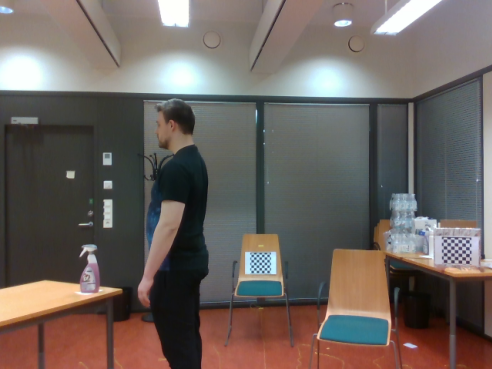
\includegraphics[width=\textwidth]{fig/5/rgb_t_7.0.png}
        \caption{RGB frame}
    \end{subfigure}
    \hfill
    \begin{subfigure}[t]{0.3\textwidth}
        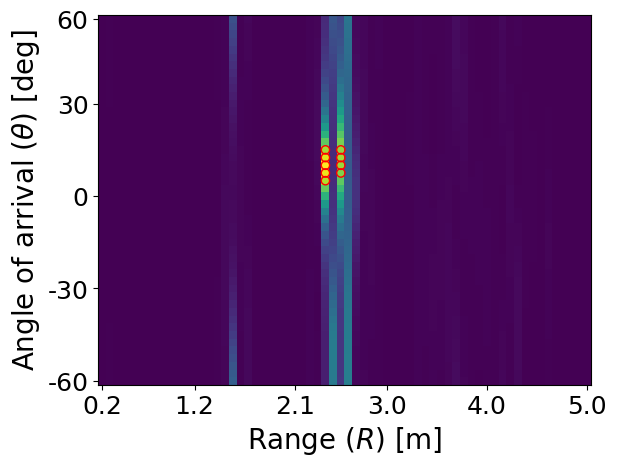
\includegraphics[width=\textwidth]{fig/5/radar_t_7.0.png}
        \caption{Radar angle-range spectrum}
    \end{subfigure}
    \caption{IR, RGB and radar frames, $\gls{time} = 7.0$.}
    \label{fig:5-frames-1}
\end{figure}

\begin{figure}
    \centering
    \begin{subfigure}[t]{0.3\textwidth}
        
\includegraphics[width=\textwidth]{fig/5/ir_t_24.0.png}
        \caption{IR frame}
    \end{subfigure}
    \hfill
    \begin{subfigure}[t]{0.3\textwidth}
        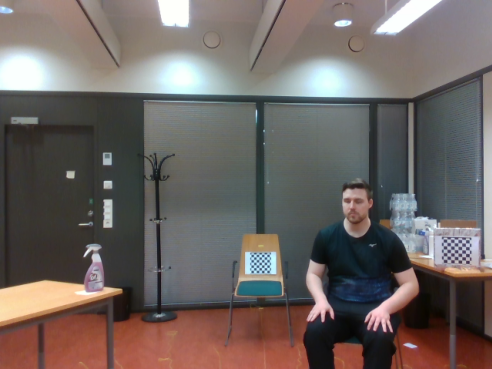
\includegraphics[width=\textwidth]{fig/5/rgb_t_24.0.png}
        \caption{RGB frame}
    \end{subfigure}
    \hfill
    \begin{subfigure}[t]{0.3\textwidth}
        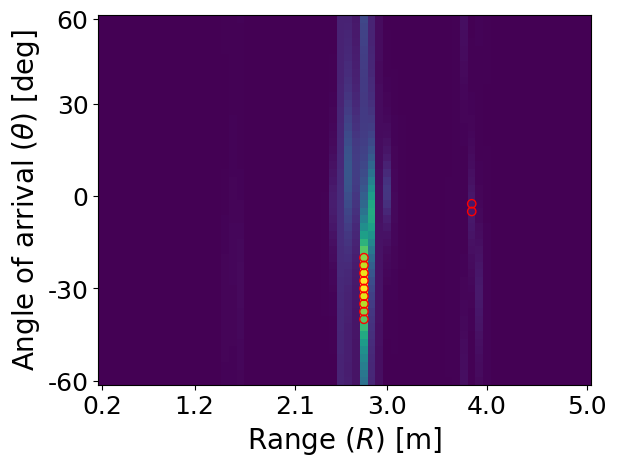
\includegraphics[width=\textwidth]{fig/5/radar_t_24.0.png}
        \caption{Radar angle-range spectrum}
    \end{subfigure}
    \caption{IR, RGB and radar frames, $\gls{time} = 24.0$.}
    \label{fig:5-frames-2}
\end{figure}

\begin{figure}
    \centering
    \begin{subfigure}[t]{0.3\textwidth}
        
\includegraphics[width=\textwidth]{fig/5/ir_t_53.0.png}
    \end{subfigure}
    \hfill
    \begin{subfigure}[t]{0.3\textwidth}
        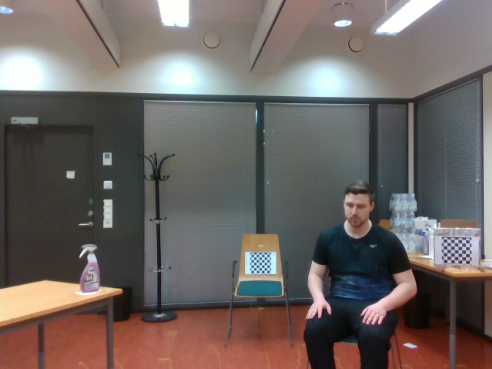
\includegraphics[width=\textwidth]{fig/5/rgb_t_53.0.png}
        \caption{RGB frame}
    \end{subfigure}
    \hfill
    \begin{subfigure}[t]{0.3\textwidth}
        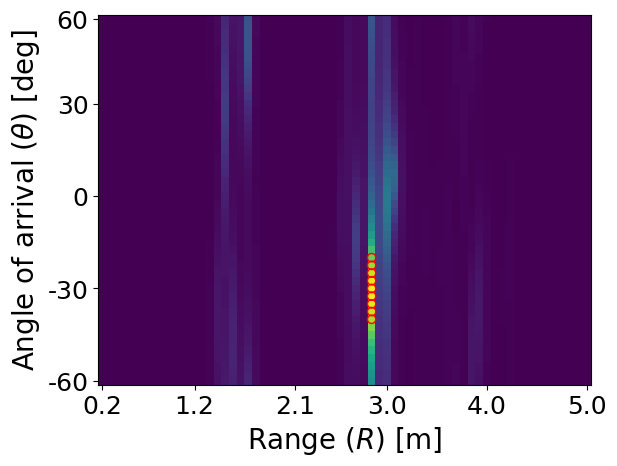
\includegraphics[width=\textwidth]{fig/5/radar_t_53.0.png}
        \caption{Radar angle-range spectrum}
    \end{subfigure}
    \caption{IR, RGB and radar frames, $\gls{time} = 53.0$.}
    \label{fig:5-frames-3}
\end{figure}

Figures \ref{fig:5-frames-1}--\ref{fig:5-frames-3} show the RGB, Radar (range-angle) and \gls{ir} frames
corresponding to different times. By looking at the frames, there seems to be high correlation between
the angle of the target, thus it can be concluded that the data is well synchronized.

\section{Data labelling}
The data can be semi-automatically labelled during testing.
Using this method, considerable effort must be made in planning the set of performed activities,
which makes the performance less natural.
Automatic activity recognition using i.e. RGB video based methods could also be used to produce the activity labels
in post-processing.
The generated labels could then be used as ground-truth information for the other sensors in machine learning algorithms.

The format of the activity labels is very simple and because the data sources are time synchronized and the frame/sampling rates are known,
it is easy to map the activities and data frames based on the time stamps and activity labels.
The data labelling can therefore be considered sufficient.

\section{Data structuring}
Each recording is stored in a single directory.
The software \gls{cli} provides a way to determine the name of the directory.
The directory names can thus be used as unique identifiers to the recordings,
and additional data such as person or room information can be mapped to the recordings using the directory names.

Under each directory, the files have consistent naming and the output from each sensor is stored in a separate file.
This makes it easy to pick and choose used sensors and minimizes the amount of data that has to be loaded into memory
for processing the output of a single sensor.

The data in the output files is unprocessed raw data from the sensors.
As a downside, lots of post-processing may be required but as an upside, no information is lost.
The structuring of the data, in the autor's opinion, is good.

\section{Metadata}
The recorded metadata considers only the sensor characteristics.
The metadata file is easy to parse programmatically as it follows the YAML syntax.
Sufficient parameter information is provided for processing the data.
Thus, the metadata can be considered sufficient.

\section{Extensibility of the system}
The system is easy to extend to include new sensors.
A recorder submodule must be written for each added sensor,
and the sensor must be added as a source to the recroded submodule.

The system was written using a very crude proceduric model.
Any well-established programming patterns were not followed.
This may have had negative effects on extensibility of the code.
Considering the module interfaces for the subprograms may have been worth considering.
Instead of passing constant strings as signals to control the program,
the signaling could have been abstracted to functions.

\section{Stability of the system}
In use, the system proved to be slightly instabile.
Sometimes after starting the software,
the recording never started as the system froze at some point of the initialization.
Power-cycling the radar device fixed the issue,
but this instability made the system much slower to use.

Effort should be made to fix the issue.
Since the issue was fixed by power-cycling the radar device,
the issue is likely related to not sending the correct commands to the radar device.
Because the issue did not occur every time,
it may also be related to parallelization.

\section{Radar data quality}
\label{sec:5-radar-spectrum-issues}
When processing the radar data, it was noticed that sometimes the range-angle spectrum
becomes extremely noisy. Figure \ref{fig:bad-radar-example} shows an example.
It may be worth investigating if using the two transmitter switching to increase the virtual number of receivers would alleviate this issue.

\begin{figure}[h]
    \centering
    \begin{subfigure}[t]{0.49\textwidth}
        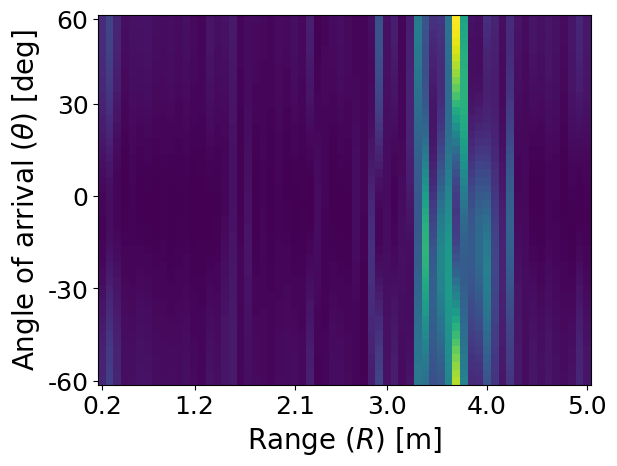
\includegraphics[width=\textwidth]{fig/5/bad-spectrum-example-radar.png}
        \caption{Radar angle-range spectrum.}
    \end{subfigure}
    \hfill
    \begin{subfigure}[t]{0.49\textwidth}
        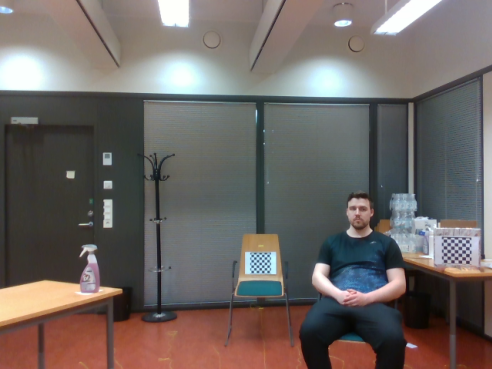
\includegraphics[width=\textwidth]{fig/5/bad-spectrum-example-rgb.png}
        \caption{Corresponding RGB image.}
    \end{subfigure}
    \caption{Example of a very noisy radar range-angle spectrum.}
    \label{fig:bad-radar-example}
\end{figure}